\chapter{Training Experience}\label{cha:report}

All groups should submit a complete but fairly concise (30-50 page) report on the project. This very same document is also written in the format expected by the DEIE under UGPs.

\section{Contents}\label{sec:report-contetns}

Report should contains the following.
\begin{itemize}
	\item Title Page
	\item Abstract
	\item Preface
	\item Acknowledgements
	\item Table of Content
	\item Acronyms (optional)
	\item List of Tables
	\item List of Figures
	\item Chapters
		\begin{itemize}
			\item Introduction
			\item Other Chapters
			\item \ldots
			\item Conclusions
		\end{itemize}
	\item Appendices
	\item Bibliography
\end{itemize}

\subsection{Introduction - The First Chapter}
The Chapter 1, ''Introduction''  may include similar to following contents.
\begin{itemize}
	\item Background of the Problem.
	\item Problem Statement
	\item Objectives and Scope
	\item Research Methodology
	\item Time Plan and Required Resources
\end{itemize}


\subsection{Other Chapters}

Must be well organized to systematically provide essential information regarding the project.

\subsection{Conclusions - The Last Chapter}

Final chapter of the report usually contains the summary of results and logical conclusions together with the suggestions for future developments.

\subsection{Appendices}

An appendix  is a section at the end of a book which includes supplementary information which may be of interest 
or use to the reader. Appendices are also used to support the qualifications of the author, and to increase the credibility of the publication.

\subsection{Bibliography}

Important points to remember on Bibliography.\\

\begin{itemize}
   \item You may use alternative name References.
   \item List down all bibliography items in alphabetical order of the first authors' name. 
   \item Each bibliography must be referred to in the text at appropriate places.
   \item refer bibliography by using number. \\
   \texttt{At present 457 out of best 500 super computers use operating systems of Linux family [2]. Many applications of Linux clusters computing can be found in [1], [4], [12] and [23]. 
   }
   \item You may opted to refer by using author name(s) and year of publication.\\
   \texttt{At present 457 out of best 500 super computers use operating systems of Linux family (Silva and Perera, 1999). Many applications of Linux clusters computing can be found in many recent publications (Silva and Perera, 1999; Benten et.al, 2005; Glica and Mirek, 2010a, Glica and Mirek, 2010b). Recently, the worst case scenario was discussed by Federmann and Bothelamous (2009) in great detail but failed to address the effect of nonlinearities on PCA.
   }
\end{itemize}
 

\section{Format}
 
\begin{itemize}
 \item Every formating aspect must have a very good reason.
 \item All formatting aspects must be perfectly consistent through out the report. 
\end{itemize}


\subsection{Documents}
Divided into chapters, chapters are numbered using arabic letters (1, 2, 3,..), each chapter starts at a new page
Chapters can be devied into sections (eg. for chapter 1 sections 1.1, 1.2, 1.3 ..). Sections can be divided into subsections (eg. 1.1.1, 1.1.2, 1.1.3, ..). Subsections are also can be divided into sub-subsections but do not use numbering.

\subsubsection{Subsubsection}
This way you may have subsubsections.

\subsection{Page}
A4, Portrait, all margins 1 inch, Gutter 0.25in, Header 0.25in, Footer 0.25in, Single Sided\\
Numbered consecutively starting from the first page of the main text through to the end of the report. Use small roman letters (i, ii, iii, iv) starting with the Preface (except Title Page and Abstract).
 
\subsection{Font}
Text: Times New Roman, Normal,12pt\\
Other effects such as underline, italic, .. can be used as appropriate.

\subsection{Paragraph}
Single Line Spacing, Justified, First line indented by 0.5in (except the first paragraph of the chapter)

\subsection{Equations}
All equations must be centered and aligned when multi-line. Number them right justified as (Chapter Number.Equation Number). \\
When necessary cite equations as for example Eq.\eqref{e:barwq} and Eq.(\ref{e:ymxc}).


\begin{equation}\label{e:barwq1}\begin{split}
H_c&=\frac{1}{2n} \sum^n_{l=0}(-1)^{l}(n-{l})^{p-2}
\sum_{l _1+\dots+ l _p=l}\prod^p_{i=1} \binom{n_i}{l _i}\\
&\quad\cdot[(n-l )-(n_i-l _i)]^{n_i-l _i}\cdot
\Bigl[(n-l )^2-\sum^p_{j=1}(n_i-l _i)^2\Bigr].
\end{split}\end{equation}

\begin{equation}\label{e:barwq}\begin{split}
H_c&=\frac{1}{2n} \sum^n_{l=0}(-1)^{l}(n-{l})^{p-2}
\sum_{l _1+\dots+ l _p=l}\prod^p_{i=1} \binom{n_i}{l _i}\\
&\quad\cdot[(n-l )-(n_i-l _i)]^{n_i-l _i}\cdot
\Bigl[(n-l )^2-\sum^p_{j=1}(n_i-l _i)^2\Bigr].
\end{split}\end{equation}

\begin{equation}\label{e:ymxc}
y = mx+c_1 + mx^2+c_2
\end{equation}

\subsection{Figures}
Figures (graphs, block diagrams, .. etc) are independent objects by nature i.e. figures should be self explanatory and understood by readers. Each figure must be numbered as Figure ChapterNumber.FigureNumber, cited and have a caption. Also should appear after citation. Good practice is to put figures in top or bottom of the page. Cite figures in the text as Figure \ref{fig:losscons}.


\begin{figure}[hbt]
        \begin{center}
                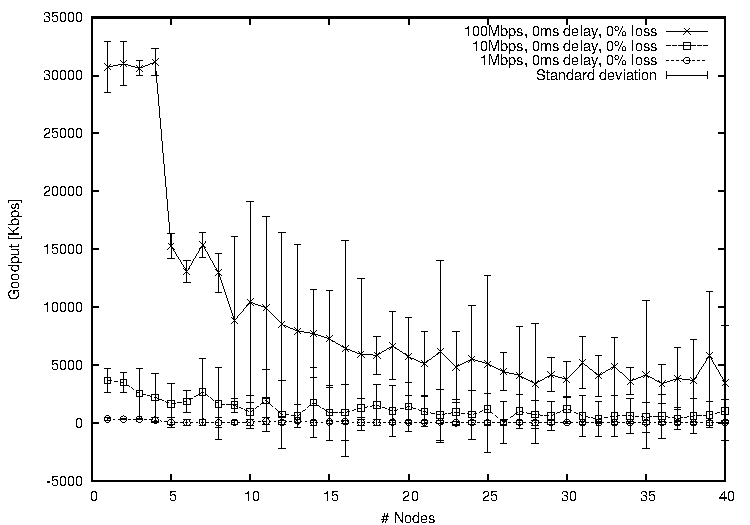
\includegraphics[width=0.9\textwidth]{01_chapters/02/figs/1000-100000_0_0.pdf}
        \end{center}
        \caption{1 - 100Mbps, 0ms delay, 0\% loss consolidated graph}
        \label{fig:losscons}
\end{figure}

 
\subsection{Tables}

Tables also are independent objects by nature. Each table must be numbered as Table ChapterNumber.TableNumber, cited and have a caption. Also should appear after citation. Good practice is to put tables in top or bottom of the page. Cite tables in the text as Table \ref{tb:sampletable}.

\begin{table}[tb]
\caption{This is an example for a table in latex.}
\label{tb:sampletable}

\begin{center}
\begin{tabular}{l|l|l}
 Name						&	Age		&	Tel \\
\hline
 Marasinghe X.Y.		& 22			&	0777-150-150\\
 \hline
 Singhemara X.Y.		& 33			&  0777-250-250\\
\end{tabular}
\end{center}
\end{table}


\subsection{Bullets and Numbering}

\subsection{Numbering}
 
 
 \begin{enumerate}
  \item Level 1
  \item Level 1
  		\begin{enumerate}
  		 \item Level2
  		 \item Level 2
  		 		\begin{enumerate}
  		 		\item Level 3
  		 		\item Level 3
  				\end{enumerate}
  		\end{enumerate}
 \item Level 1
 \end{enumerate}
 
 \subsection{Bullets}
 
\begin{itemize}
  \item Level 1
  \item Level 1
  		\begin{itemize}
  		 \item Level2
  		 \item Level 2
  		 		\begin{itemize}
  		 		\item Level 3
  		 		\item Level 3
  				\end{itemize}
  		\end{itemize}
 \item Level 1
 \end{itemize}
 
 \subsection{Description}
 
 \begin{description}
  \item [Step 1] Open a text editor such as Emacs.
  \item [Step 2] Close WYSIWYG editors
  \item [Step 3] Goto Step 1.
 \end{description}
 
 
 \subsection{Mixed}
 
 \begin{enumerate}
  \item Level 1
 \item Level 1
  		\begin{itemize}
  		 \item Level2
  		 \item Level 2
  		 		\begin{enumerate}
  		 		\item Level 3
  		 		\item Level 3
  				\end{enumerate}
  		\end{itemize}
 \item Level 1
 \end{enumerate}

\section{Notes on Writing}
\begin{itemize}
 \item Simplest possible English.
 \item Third Person
 \item Simple Present Tense (Passive Voice): Explain the project
 \item Present Perfect Tense (Passive Voice): Explain experiments
 \item Past Perfect Tense: Use only if you can not live without.
 \item Consistency (e.g. symbols used, format, ..)
 %\item 
\end{itemize}



%%%%%%%%%%%%%%%%%%%%%%%%%%%%%%%%%%%%%%%%%%%%%%%%%%%%%%%%%%%%%%%%%%%%%%%%%%%%%%%%%%%%%%%%%%%%%%%%%%
%%%%%%%%%%% END OF FILE
%%%%%%%%%%%%%%%%%%%%%%%%%%%%%%%%%%%%%%%%%%%%%%%%%%%%%%%%%%%%%%%%%%%%%%%%%%%%%%%%%%%%%%%%%%%%%%%%%%
